% ==========================================================================
% % Copyright (C) 2016 Dr. Alejandro Pina Ortega
% %
% % Licensed under the Apache License, Version 2.0 (the "License");
% % you may not use this file except in compliance with the License.
% % You may obtain a copy of the License at
% %
% %      http://www.apache.org/licenses/LICENSE-2.0
% %
% % Unless required by applicable law or agreed to in writing, software
% % distributed under the License is distributed on an "AS IS" BASIS,
% % WITHOUT WARRANTIES OR CONDITIONS OF ANY KIND, either express or implied.
% % See the License for the specific language governing permissions and
% % limitations under the License.
% ==========================================================================

%----------------------------------------------------------------------------------------
%	PACKAGES AND OTHER DOCUMENT CONFIGURATIONS
%----------------------------------------------------------------------------------------

\documentclass{tufte-book} % Use the tufte-book class which in turn uses the tufte-common class

\hypersetup{colorlinks} % Comment this line if you don't wish to have colored links

\usepackage{microtype} % Improves character and word spacing

\usepackage{lipsum} % Inserts dummy text

\usepackage{booktabs} % Better horizontal rules in tables

\usepackage{graphicx} % Needed to insert images into the document
\graphicspath{{../../images/}} % Sets the default location of pictures
\setkeys{Gin}{width=\linewidth,totalheight=\textheight,keepaspectratio} % Improves figure scaling

\usepackage{fancyvrb} % Allows customization of verbatim environments
\fvset{fontsize=\normalsize} % The font size of all verbatim text can be changed here

\newcommand{\hangp}[1]{\makebox[0pt][r]{(}#1\makebox[0pt][l]{)}} % New command to create parentheses around text in tables which take up no horizontal space - this improves column spacing
\newcommand{\hangstar}{\makebox[0pt][l]{*}} % New command to create asterisks in tables which take up no horizontal space - this improves column spacing

\usepackage{xspace} % Used for printing a trailing space better than using a tilde (~) using the \xspace command

\newcommand{\monthyear}{\ifcase\month\or January\or February\or March\or April\or May\or June\or July\or August\or September\or October\or November\or December\fi\space\number\year} % A command to print the current month and year

\newcommand{\openepigraph}[2]{ % This block sets up a command for printing an epigraph with 2 arguments - the quote and the author
\begin{fullwidth}
\sffamily\large
\begin{doublespace}
\noindent\allcaps{#1}\\ % The quote
\noindent\allcaps{#2} % The author
\end{doublespace}
\end{fullwidth}
}

\newcommand{\blankpage}{\newpage\hbox{}\thispagestyle{empty}\newpage} % Command to insert a blank page

\usepackage{makeidx} % Used to generate the index
\makeindex % Generate the index which is printed at the end of the document

%----------------------------------------------------------------------------------------
%	BOOK META-INFORMATION
%----------------------------------------------------------------------------------------

%\title{UFFEMA: \newline Unified Framework for Electric Machine Analysis \newline REFERENCE MANUAL VERSION 0.1} % Title of the book

%\author{UFFEMA Developers} % Author

%\publisher{Dr. A. J. Pi\~{n}a Ortega} % Publisher

%----------------------------------------------------------------------------------------

\begin{document}

\frontmatter

\begin{titlepage}
\begin{fullwidth}

	\centering
%	\includegraphics[width=0.15\textwidth]{example-image-1x1}\par\vspace{1cm}
	{\LARGE \textit{UFFEMA DEVELOPERS} \par}
	\vspace{5cm}
	{\fontsize{40}{50}\selectfont\bfseries UFFEMA:\par}
	{\fontsize{30}{40}\selectfont\itshape\bfseries Unified Framework for Electric Machine Analysis\par}
	\vspace{2cm}
	{\LARGE\flushright  REFERENCE MANUAL VERSION $0.1$\par}
	\vspace{7cm}
	{\Large\itshape Dr. A. J. Pi\~{n}a Ortega\par}

	\vfill

% Bottom of the page
	{\large \today\par}

\end{fullwidth}
\end{titlepage}

%----------------------------------------------------------------------------------------
%	EPIGRAPH
%----------------------------------------------------------------------------------------

%\thispagestyle{empty}
%\openepigraph{Quotation 1}{Author, {\itshape Source}}
%\vfill
%\openepigraph{Quotation 2}{Author}
%\vfill
%\openepigraph{Quotation 3}{Author}

%----------------------------------------------------------------------------------------

%\maketitle % Print the title page

%----------------------------------------------------------------------------------------
%	COPYRIGHT PAGE
%----------------------------------------------------------------------------------------

\newpage
\begin{fullwidth}
~\vfill
\thispagestyle{empty}
\setlength{\parindent}{0pt}
\setlength{\parskip}{\baselineskip}
Copyright \copyright\ \the\year\ Dr. A. J. Pi\~{n}a Ortega

\par\smallcaps{Powered by UFFEMA DEVELOPERS}

\par\smallcaps{\url{https://github.com/ajpina/uffema}}

\par Licensed under the Apache License, Version 2.0 (the ``License''); you may not
use this file except in compliance with the License. You may obtain a copy
of the License at \url{http://www.apache.org/licenses/LICENSE-2.0}. Unless
required by applicable law or agreed to in writing, software distributed
under the License is distributed on an \smallcaps{``AS IS'' BASIS, WITHOUT
WARRANTIES OR CONDITIONS OF ANY KIND}, either express or implied. See the
License for the specific language governing permissions and limitations
under the License.\index{license}

\par\textit{First printing, \monthyear}
\end{fullwidth}

%----------------------------------------------------------------------------------------

\tableofcontents % Print the table of contents

%----------------------------------------------------------------------------------------

\listoffigures % Print a list of figures

%----------------------------------------------------------------------------------------

\listoftables % Print a list of tables

%----------------------------------------------------------------------------------------
%	DEDICATION PAGE
%----------------------------------------------------------------------------------------

%\cleardoublepage
%~\vfill
%\begin{doublespace}
%\noindent\fontsize{18}{22}\selectfont\itshape
%\nohyphenation
%Dedicated to my family and friends.
%\end{doublespace}
%\vfill
%\vfill

%----------------------------------------------------------------------------------------
%	INTRODUCTION
%----------------------------------------------------------------------------------------

\cleardoublepage
\chapter*{Introduction} % The asterisk leaves out this chapter from the table of contents

The Unified Framework for Electric Machine Analysis describes with parameters the geometries found in electric machines. Although it would be unrealistic cover all possible shapes or all small details that creative designers put into their models when trying to enhance specific machine behaviours, this document will try to gather the most common geometries of the most common rotating electric machines.

This reference should become a living document that will be incorporating features and evolving such as electric machines have done it since their conception.   

\begin{figure*}[h]
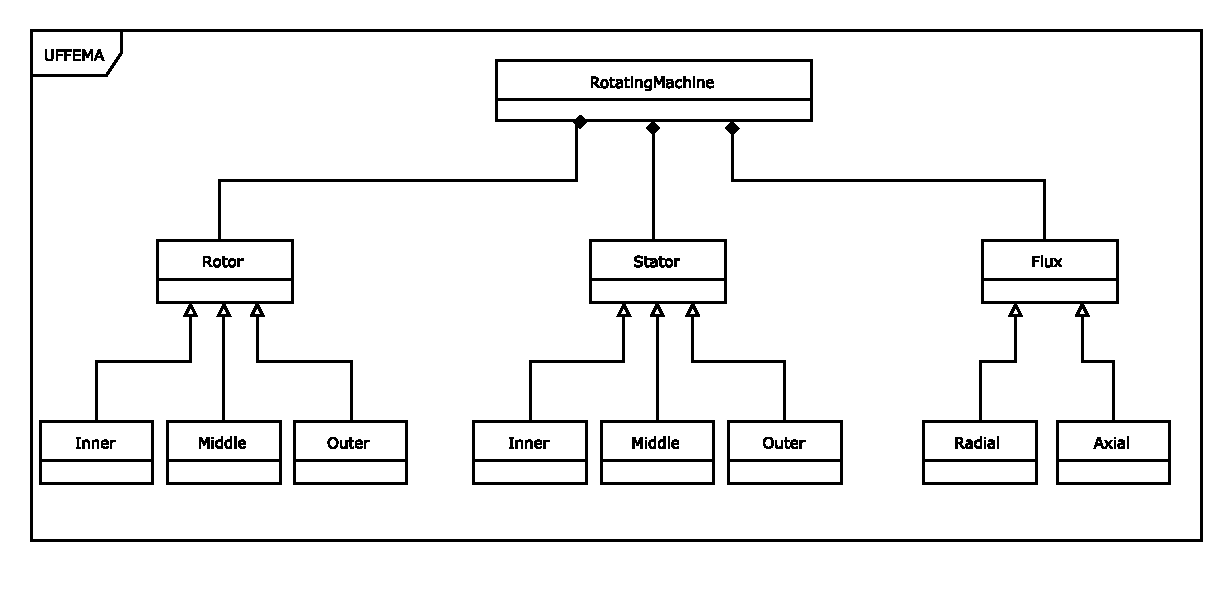
\includegraphics[width=\linewidth]{Overview.pdf}
\caption{ Composition of rotating electric machines 
%\emph{Notice that this figure takes up the full page width.}
}
\label{fig:overview}
\end{figure*}

Throughout this document, rotating electric machines will be referred simply as electric machines, so the perspicacious readers will probably complain on that terminology since linear machines or transformers are not treated here.  Hence, we apologise for appropriating the definition.     

The abstraction of Figure \ref{fig:overview} shows the first level of simplicity of electric machines and the sort of relationships will be found along this manual. From this definition, a \textit{RotatingMachine} must have one or more \textit{Rotor}, \textit{Stator} as well as \textit{Flux}. Either \textit{Rotor} or \textit{Stator} might be of \textit{Inner}, \textit{Middle} or \textit{Outer} construction.

Initially, this document will be dealing with geometries that can be included on machines of \textit{Radial} or \textit{Axial} \textit{Flux}.

\begin{figure*}[h]
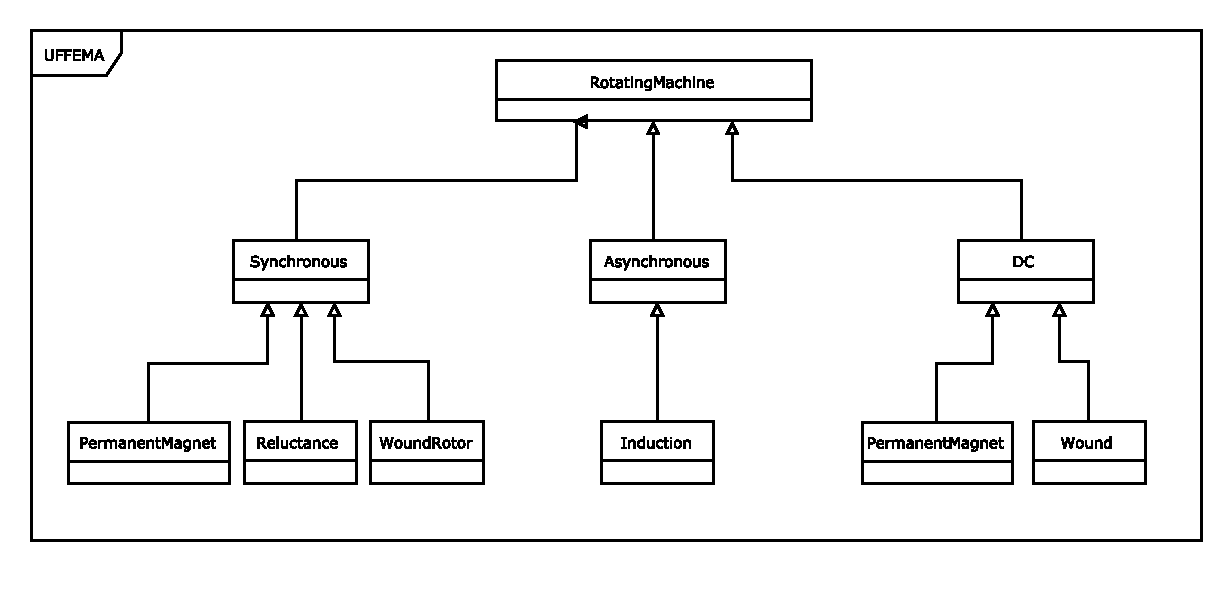
\includegraphics[width=\linewidth]{RotatingMachine.pdf}
\caption{Classification of rotating electric machines 
%\emph{Notice that this figure takes up the full page width.}
}
\label{fig:fullfig}
\end{figure*}

Citation example \cite{Tufte2001}, notice how the citation is in the margin. This is an example of how to add something to the index at the end of the document.\index{citation}

\newthought{Example of} the \texttt{newthought} command for starting new sections. Typography examples: \allcaps{all caps} and \smallcaps{small caps}.

%------------------------------------------------

\section{Synchronous}

\section{Asynchronous}

\section{DC}

\lipsum[1] 

\begin{marginfigure}
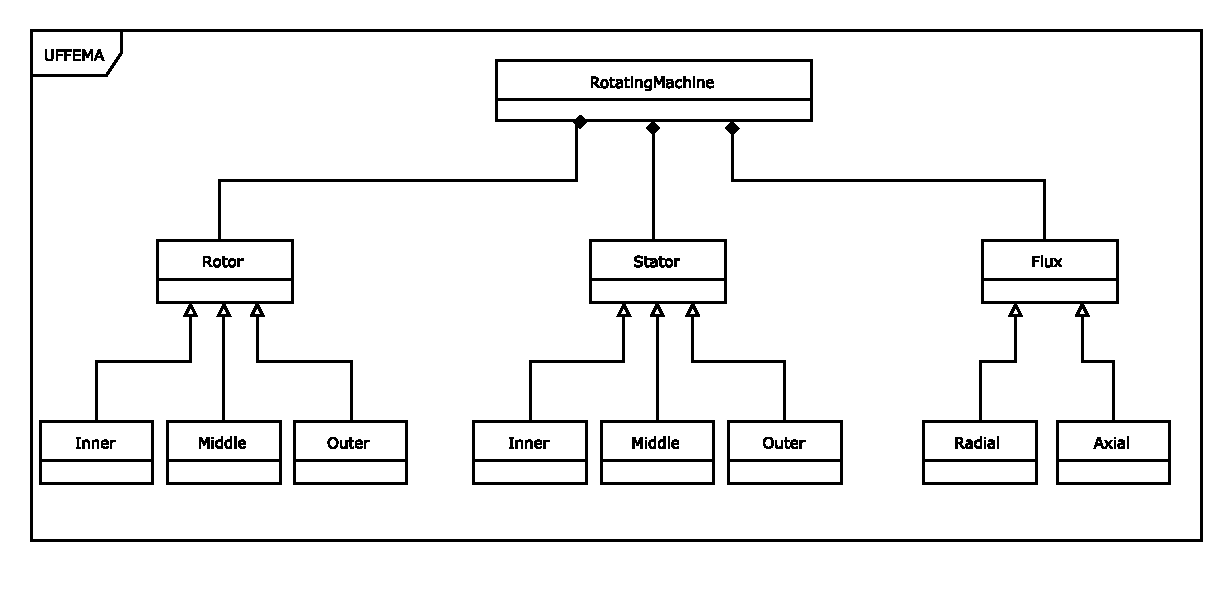
\includegraphics[width=\linewidth]{Overview.pdf}
\caption{This is a margin figure. The helix is defined by $x = \cos(2\pi z)$, $y = \sin(2\pi z)$, and $z = [0, 2.7]$. The figure was drawn using Asymptote (\url{http://asymptote.sf.net/}).}
\label{fig:marginfig}
\end{marginfigure}

\lipsum[2]



\lipsum[3]

%------------------------------------------------

\section{Tables} \marginnote{This is a random margin note. Notice that there isn't a number preceding the note, and there is no number in the main text where this note was written. Use \texttt{sidenote} to use a number.}

\lipsum[4]

\begin{table} % Add the following just after the closing bracket on this line to specify a position for the table on the page: [h], [t], [b] or [p] - these mean: here, top, bottom and on a separate page, respectively
\centering % Centers the table on the page, comment out to left-justify
\begin{tabular}{l c c c c c} % The final bracket specifies the number of columns in the table along with left and right borders which are specified using vertical bars (|); each column can be left, right or center-justified using l, r or c. To specify a precise width, use p{width}, e.g. p{5cm}
\toprule % Top horizontal line
& \multicolumn{5}{c}{Growth Media} \\ % Amalgamating several columns into one cell is done using the \multicolumn command as seen on this line
\cmidrule(l){2-6} % Horizontal line spanning less than the full width of the table - you can add (r) or (l) just before the opening curly bracket to shorten the rule on the left or right side
Strain & 1 & 2 & 3 & 4 & 5\\ % Column names row
\midrule % In-table horizontal line
GDS1002 & 0.962 & 0.821 & 0.356 & 0.682 & 0.801\\ % Content row 1
NWN652 & 0.981 & 0.891 & 0.527 & 0.574 & 0.984\\ % Content row 2
PPD234 & 0.915 & 0.936 & 0.491 & 0.276 & 0.965\\ % Content row 3
JSB126 & 0.828 & 0.827 & 0.528 & 0.518 & 0.926\\ % Content row 4
JSB724 & 0.916 & 0.933 & 0.482 & 0.644 & 0.937\\ % Content row 5
\midrule % In-table horizontal line
\midrule % In-table horizontal line
Average Rate & 0.920 & 0.882 & 0.477 & 0.539 & 0.923\\ % Summary/total row
\bottomrule % Bottom horizontal line
\end{tabular}
\caption{Table caption text} % Table caption, can be commented out if no caption is required
\label{tab:template} % A label for referencing this table elsewhere, references are used in text as \ref{label}
\end{table}

%----------------------------------------------------------------------------------------

\mainmatter

%----------------------------------------------------------------------------------------
%	CHAPTER 1
%----------------------------------------------------------------------------------------

\chapter{Permanent Magnet Machines}
\label{ch:1}

\begin{figure*}[h]
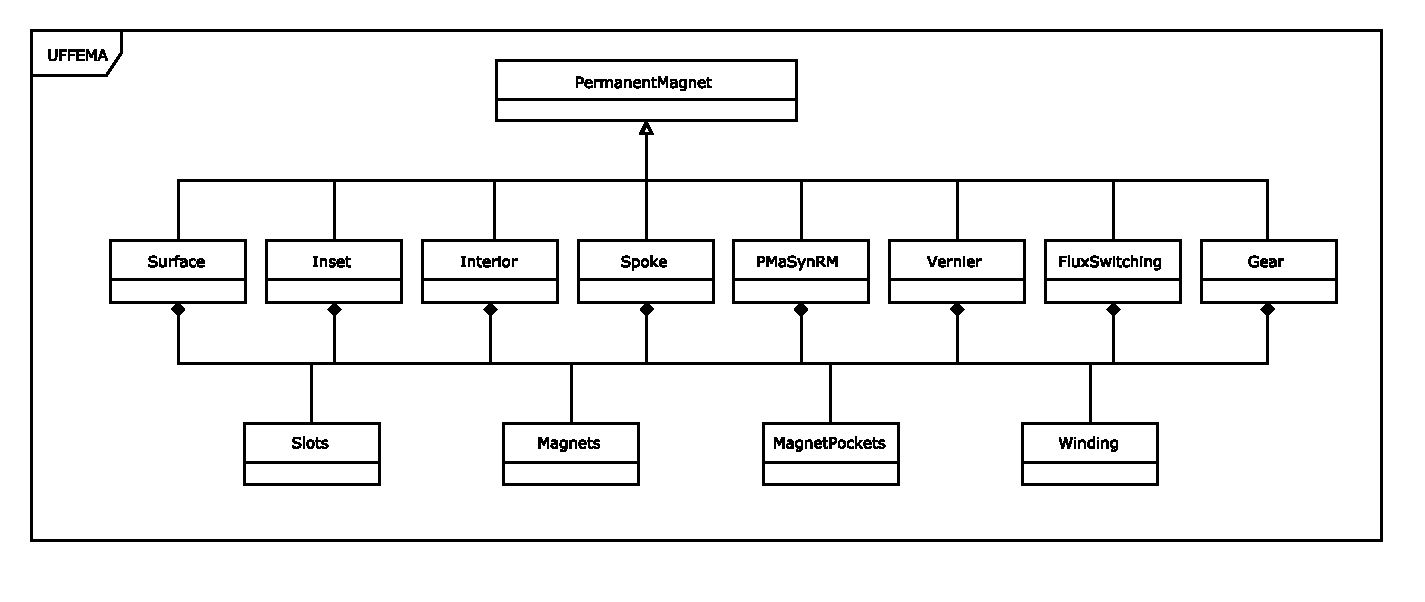
\includegraphics[width=\linewidth]{PermanentMagnet.pdf}
\caption{This graph shows $y = \sin x$ from about $x = [-10, 10]$.
\emph{Notice that this figure takes up the full page width.}}
\label{fig:fullfig}
\end{figure*}
%------------------------------------------------

\section{Section 1 - Fullwidth Environment Example}

\begin{fullwidth}
\lipsum[5]
\end{fullwidth}

\subsection{Subsection 1}

\lipsum[6-7]

\subsection{Subsection 2}

\lipsum[7-8]

%------------------------------------------------

\section{Section 2}

\subsection{Subsection 1}

\lipsum[9-10]

\subsection{Subsection 2}

\lipsum[11-12]

%----------------------------------------------------------------------------------------
%	CHAPTER 2
%----------------------------------------------------------------------------------------

\chapter{Chapter 2 Title}
\label{ch:2}

\lipsum[13-20]

%----------------------------------------------------------------------------------------

\backmatter

%----------------------------------------------------------------------------------------
%	BIBLIOGRAPHY
%----------------------------------------------------------------------------------------

\bibliography{uffema-refman-bib} % Use the bibliography.bib file for the bibliography
\bibliographystyle{plainnat} % Use the plainnat style of referencing

%----------------------------------------------------------------------------------------

\printindex % Print the index at the very end of the document

\end{document}
